\chapter{附录}
\label{sec.appendix}

\section{校园地图}
\begin{figure}[H]
    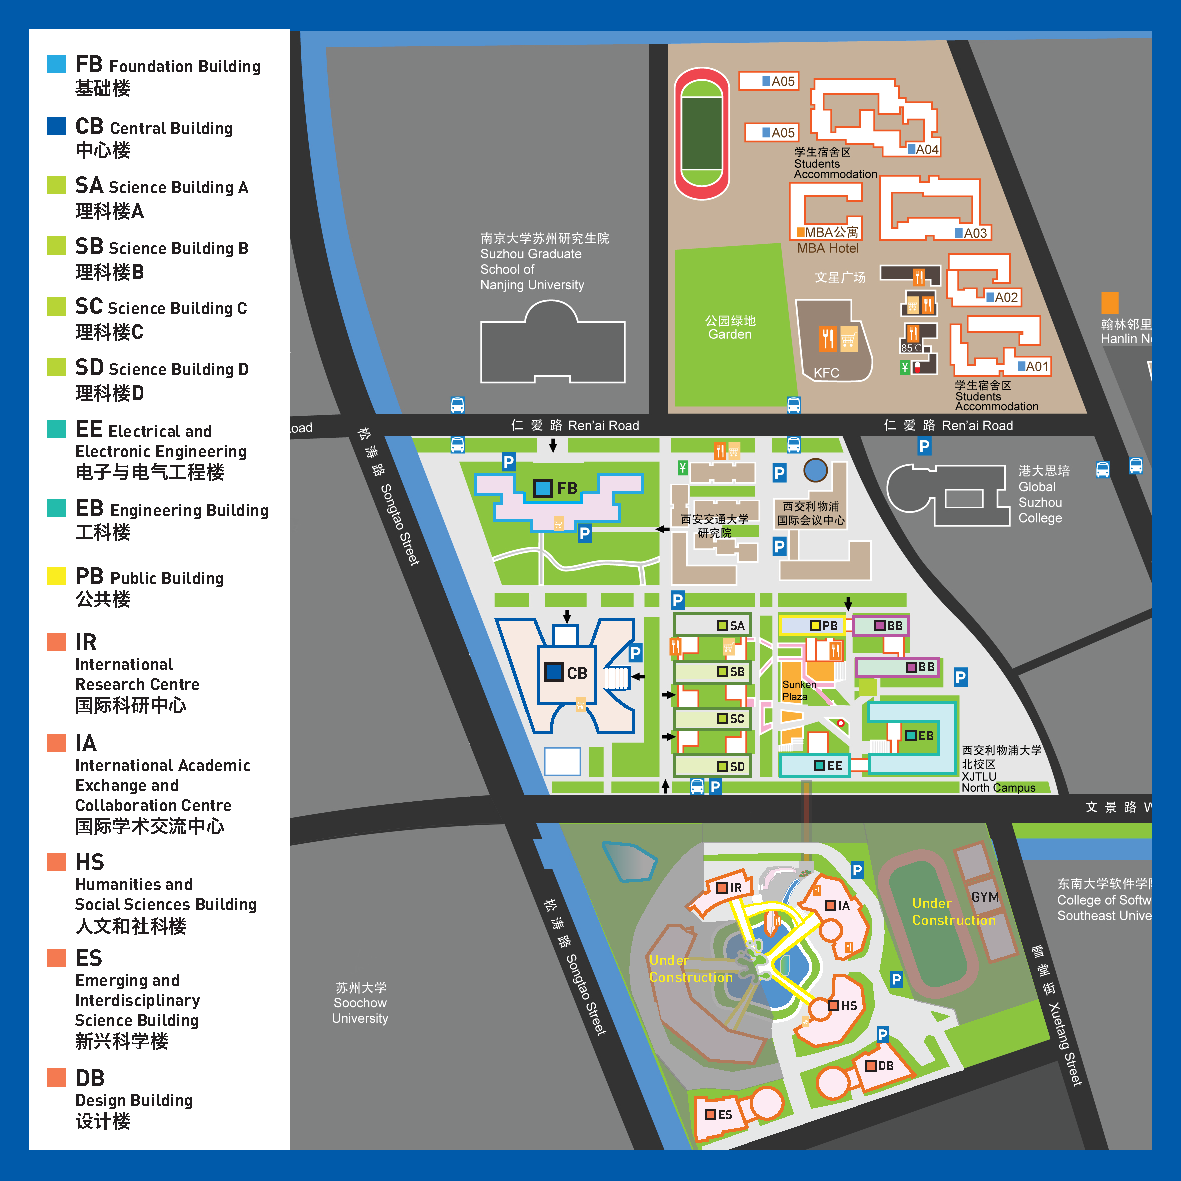
\includegraphics[width=\columnwidth]{author-folder/Kai.Wu/XJTLU-campus-map.pdf}
\end{figure}

\clearpage
\section{校历:哪天放假}
独立的校历文件可在本项目的GitHub里(\href{https://github.com/kaiwu-astro/xp_pgrs_unofficial_guide/raw/main/author-folder/Kai.Wu/Academic_Calendar-202223.pdf}{链接})找到。
\begin{figure}[H]
    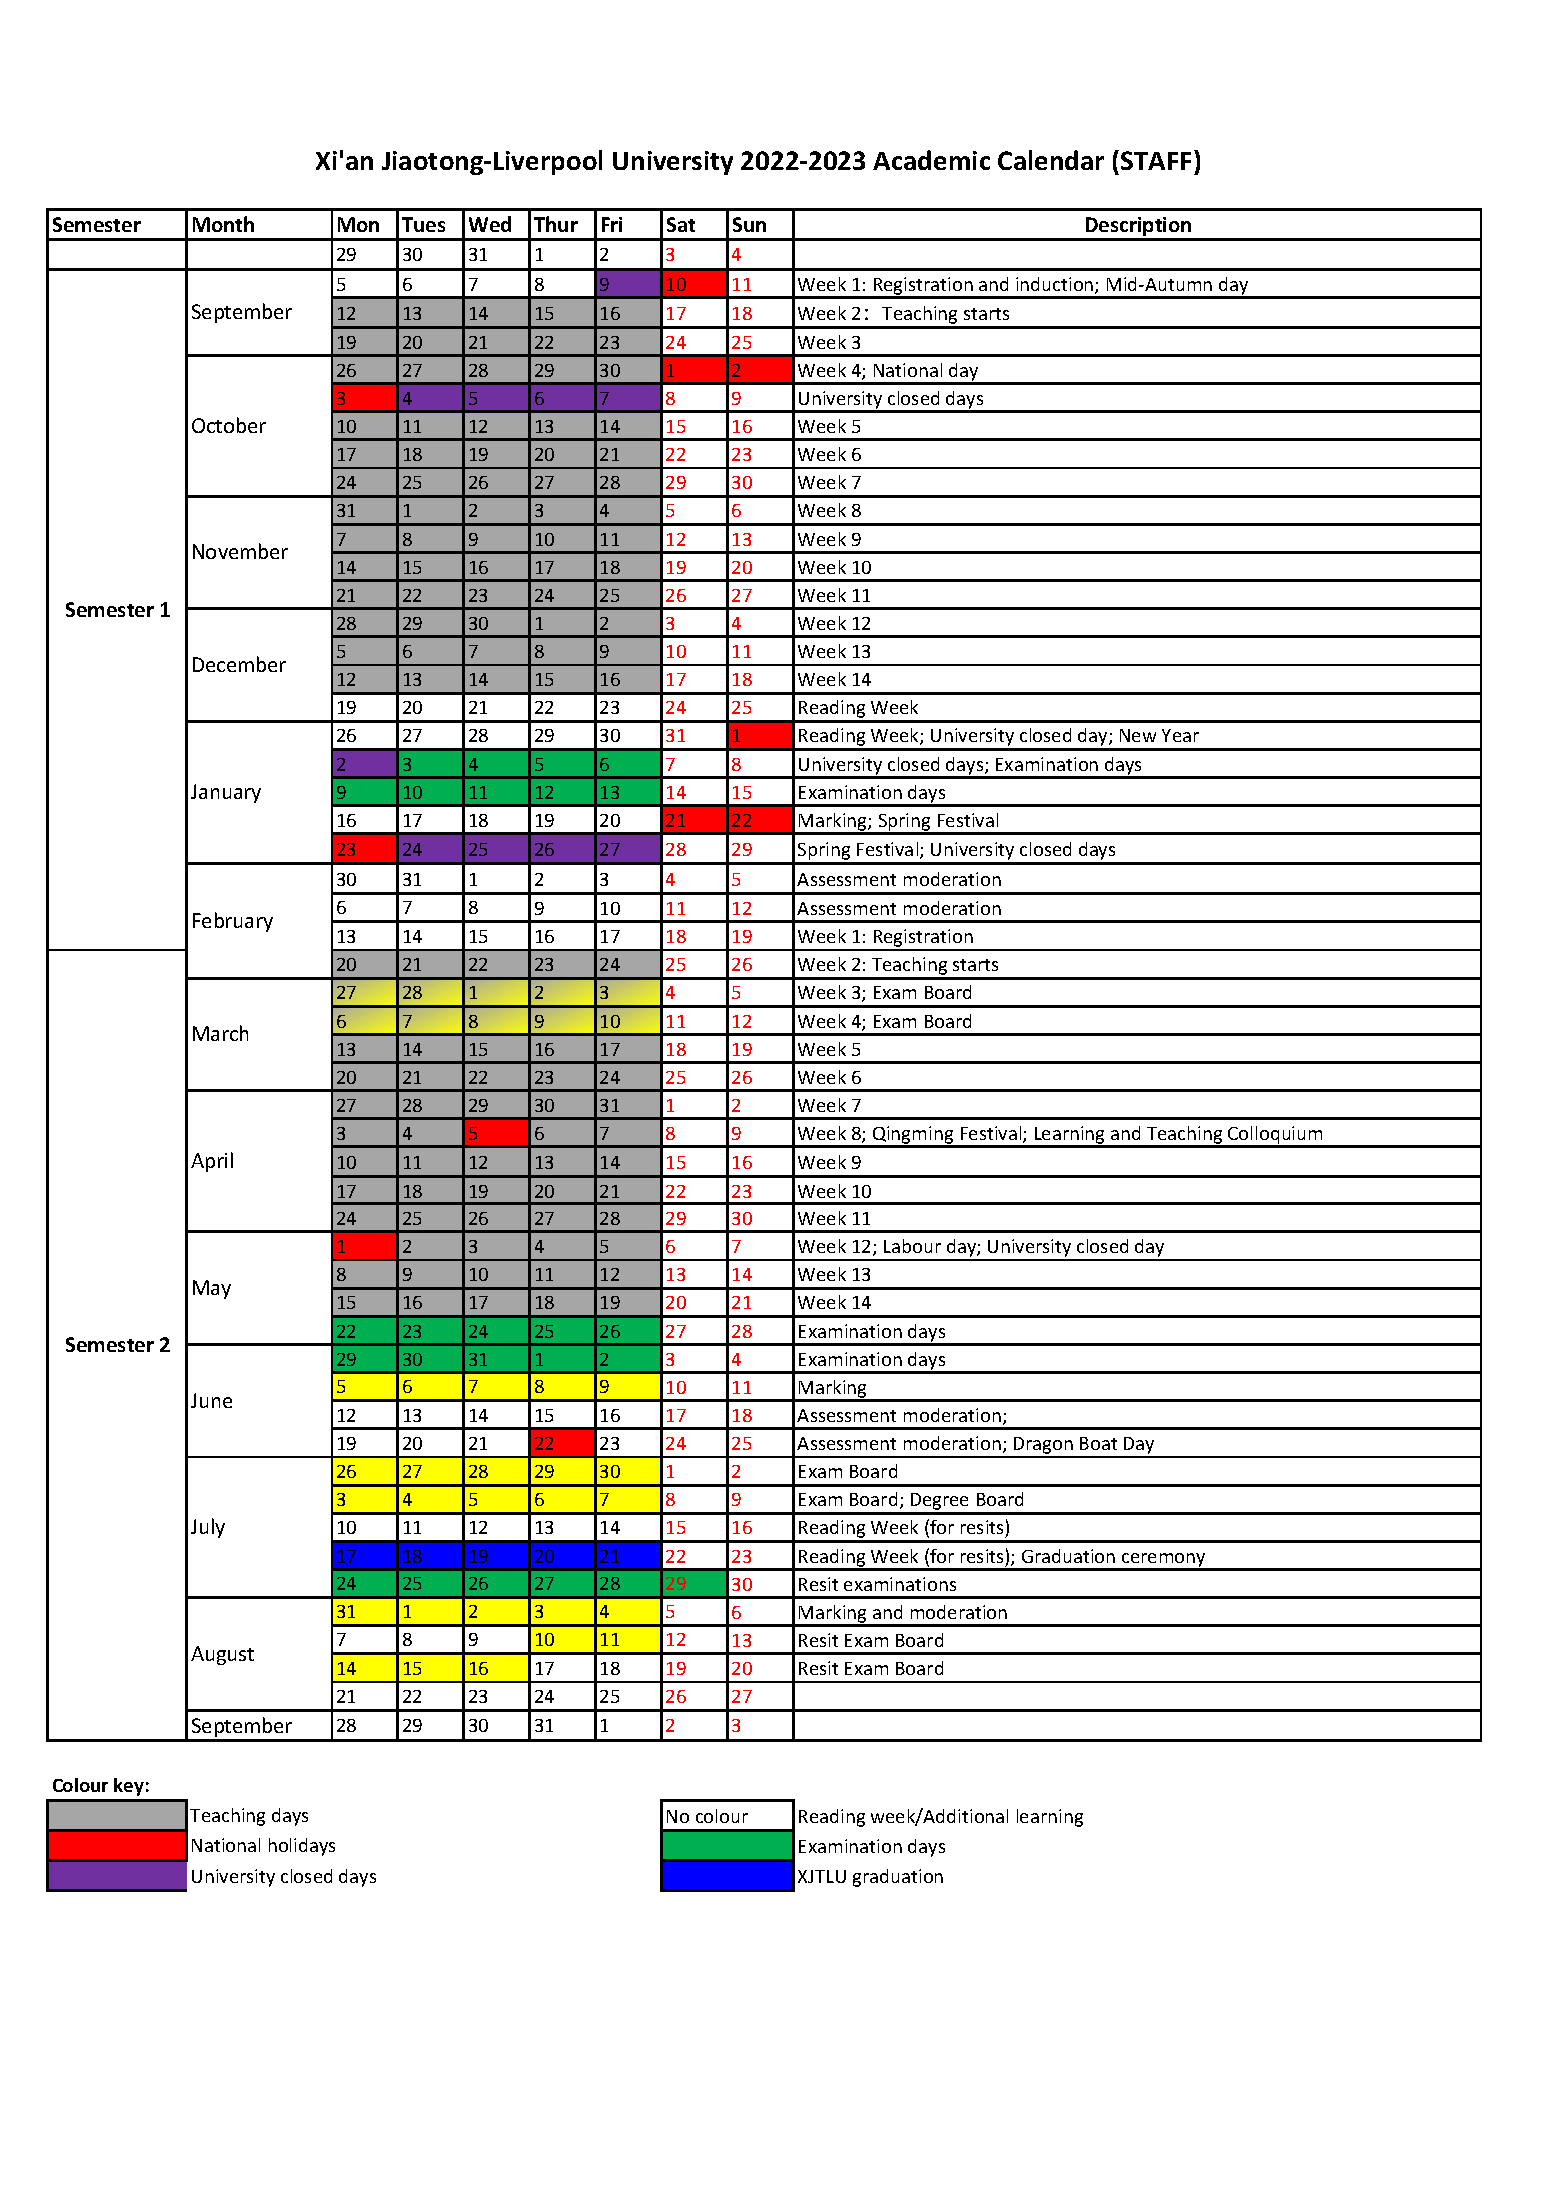
\includegraphics[width=0.9\columnwidth]{author-folder/Kai.Wu/Academic_Calendar-202223.pdf}
\end{figure}

\section{学校电话}

\begin{table}[H]
    \begin{tabular}{p{60mm}cc}
        \hline
        部门 & 电话 & 邮箱 \\ \hline
        Academic Services Office \newline 学术服务 & 8188 4754 & aso@xjtlu.edu.cn \\ \hline
        Alumni Service \newline 校友服务           & 8816 1869 & alumni@xjtlu.edu.cn \\ \hline
        Campus Management Office\newline 校园管理办公室 & 8816 1071 &  \\ \hline
        Career Service \newline 就业服务           & 8188 8308 &  \\ \hline
        IT Service Centre \newline IT服务中心      & 8816 1250 & it@xjtlu.edu.cn \\ \hline
        Library \newline 图书馆                    & 8816 1290 &  \\ \hline
        Media Service \newline 新闻线索与媒体服务    & 8816 1351/1032 & news@xjtlu.edu.cn \\ \hline
        Postgraduate Recruitment \newline 研究生招生 & 8816 1889/7111 & pgenquiries@xjtlu.edu.cn \\ \hline
        President's Office \newline 校长办公室     & 8816 1004 &  \\ \hline
        Registry \newline 教务办公室               & 8816 1230 & registry@xjtlu.edu.cn \\ \hline
        Research Management Office \newline 科研管理办公室 & 8816 1139 &  \\ \hline
        Student Onestop Centre \newline 学生一站式 & 8816 1854 & onestop@xjtlu.edu.cn \\ \hline
        XJTLU Global (Support) \newline 西浦国际 & 8897 3094/3093 & global@xjtlu.edu.cn \\ \hline
    \end{tabular}
\end{table}